\subsection{\proj Operations}
 
% Real-time monitoring systems:

\begin{wrapfigure}{!h}{3.5in}
  \vspace{-0.8cm}
  \centering
  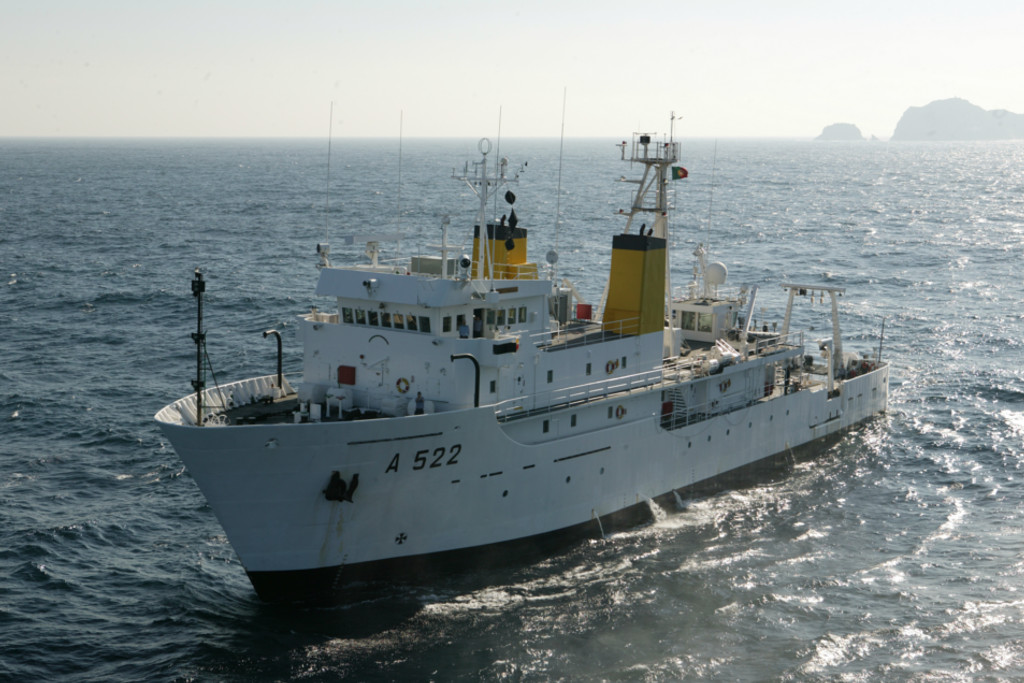
\includegraphics[scale=1.75]{fig/dom-carlos.jpg}
  \caption{A 70m research vessel, the NRP \emph{Dom Carlos} or its
    sister vessel will be available for \proje.}
  % \vspace{-0.3cm}
 \label{fig:vessel}
\end{wrapfigure}

Off shore in the \naz canyon-Berlengas area are two islands of Berlengas
and Farilho\~es part of a protected nature preserve. With special
permission we expect to be able to be based in Berlengas for a period of
3 weeks to conduct off shore operations. A small team will also be
present onboard the \inst research vessel where if needed, deployment
and recovery of assets well off shore at the boundaries of the survey
region, can be done. In addition \inst will be in a position to provide
a RHIB or a rigid boat for near-shore operations from the two islands.

\univ will provide the bulk of the robotic assets including aerial,
surface and underwater vehicles as also the team to operate them. The
team will be split between being based in Berlengas, the research vessel
and also provide remote monitoring from Porto. \soc will provide at
least one glider to operate outside the shelf to augment model
observations in the meso-scale.

\proj will leverage existing real-time monitoring capacities which were
installed and are operated by Instituto Hidrogr\'{a}fico (\inste). These
include two multi-parametric buoys with satellite transmission of hourly
data sets and two coastal tide gauges installed in the ports of \naz and
Peniche. These systems form the \naz Canyon Observatory \texttt{MONICAN}
which is a subset of the global real-time monitoring infrastructure for
the Portuguese Exclusive Economic Zone operated by \inst \kc{(MONIZEE
  infrastructure, see figure X)}. In addition, we will leverage ship
time from one of the \inst research vessels which visit the \naz area
for buoy maintenance twice yearly. \inst will provide access to this
vessel where a small \proj team will be resident, in addition to those
being housed in the Berlengas island.

Each multiparametric buoy is equipped with:

\begin{enumerate}

  \item A meteorological mast providing hourly measurements of wind speed and
    direction, air temperature, atmospheric pressure and relative
    humidity

  \item A wave sensor providing hourly measurements of standard wave parameters
    (wave spectra at the end of the deployment)

  \item A downward looking 300 kHz RDI Workhorse ADCP installed at 7 m
    depth and providing currents with $sim 2$ m resolution to about 90 m
    depth Surface temperature sensor (SBE AADI Subsurface temperature
    sensors)

\end{enumerate}  


The buoys are also equipped with fluorometers but the response of these
sensors rapidly degrades in about 1-2 weeks, after maintenance,
primarily due to biofouling.

Additional systems could also be available for \proje. A separate
project proposal was submitted at the end of 2020~\footnote{EEA Grants,
  Portugal} where a HF radar system has been proposed for the \naz area.
The system, a CODAR Seasonde with two antennas operating at 13 MHz, one
installed in \naz and the other in Peniche. A previous test of a similar
system was conducted by \inst in September--November 2011 and showed
that surface currents measurements were available for the complete area
to about 70 km from the shore with a 1 km resolution \kc{(figure)}.
 
  
\subsection{At-Sea operations}

\proj will observe the coastal ocean area of interest off of \naz, in
such a way as to improve the initialization/assimilation fields and
parameter definitions to be used in the physical and biogeochemical
models. To achieve this objective \proj will develop a strategy largely
inspired in the Rapid Environmental Assessment to navy operations
\kc{citation?}. Specifically a total of three phases (weeks 1 to 3) are
planned:


\begin{wrapfigure}{!}{4.4in}
  % \vspace{-0.5cm}
  \centering
  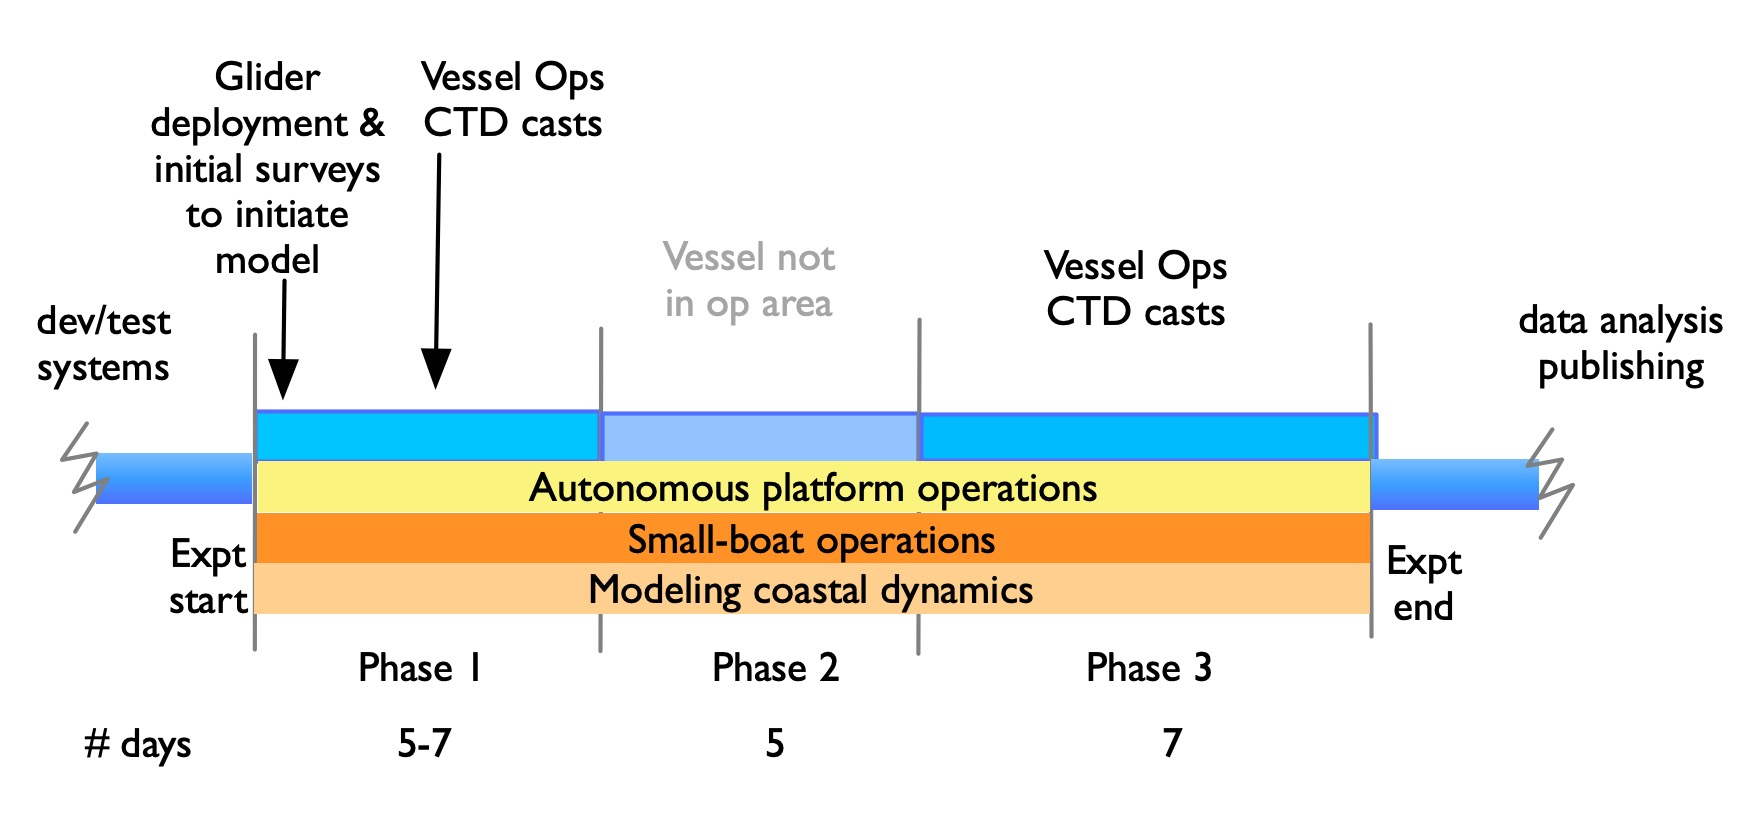
\includegraphics[scale=0.22]{fig/timelines.jpg}
  \caption{At-sea operations for \proj will be split along 4 phases.
    Phase 0 will involve glider deployments at the further reaches of
    the operations boundary. Phase 1 will commence with vessel
    operations including CTD casts, followed by Phase 2 when the vessel
    will depart the \naz operational area. Phase 3 will commence with
    the resumption of vessel ops. Autonomous platforms starting with
    gliders will be operating continuously through all phases of the
    experiment.}
  % \vspace{-0.3cm}
 \label{fig:expt-phases}
\end{wrapfigure}

 
Phase 1 (precursor survey):
 
A preliminary characterization of the geographical area of interest will
be conducted during this initial period. The precursor phase will be
preceded by the identification of the prevailing features that
characterize the coastal ocean area of interest from remote sensing
imagery and (if available) from surface currents measured by a HF radar
system. The surface data will allow to identify the main features
present in the area (in SST, Chl and turbidity and currents) and to
select a limited number of key locations in which the surface
information will be complemented by water column observations. In case
no surface data is available (because of cloud cover obstructing optical
remote sensing) the location of these points will be dictated by the
characteristics of the topography of the area, by the prevailing forcing
conditions and by previous knowledge about the primary processes.
 
The precursor survey will combine operations onboard a small boat with
operations conducted onboard a \inst hydrographic vessel that will pass
through the area during this period. 
 
During 2--3 days a small team onboard a small-boat will conduct a set of
measurements in the water column (to about 200 m depth) at the key
location point identified earlier using low cost systems \kc{this is
  vague} and other sensors of interest and water samples collected at
selected depths on those key locations. Sampling with vertical nets will
also be done at some of these positions. Part of the water samples
collected will be used to evaluate the nutrient profiles in the water
column. These samples will be analyzed at the \inst Marine Chemistry and
Pollution laboratories and will be available in about 1--2 days.
Depending on period selected for the exercise these measurements would
help to characterize the nutrient intake to upper levels associated
with intensified upwelling at the canyon head or the inputs to the
coastal ocean associated by freshwater inputs along the coast. Combined
with the information available from remote sensing images, this data will
provide the basis for the initialization of the nutrients fields in the
BGC model.
 
Part of the water samples and samples collected with a vertical net will
be used to characterize the phyto- and zoo plankton communities. These
samples will provide the basis for the initialization of the phyto and
zooplankton compartments of the BGC model.
 
At the same time the hydrographic vessel will pass on the area and
during this period will conduct a very limited number of CTD profiles
and collect vessel mounted ADCP measurements. The analysis of water
samples collected by the small boat campaign at a few locations and same
times will then be used for calibration of the CTD fluorometer and
calibrate the ADCP echo intensity data in zooplankton biomass. These
calibrations will then be used during next phase of the survey

\kc{
This data will also be used to calibrate the response of fluorometers to
be used in response
 
This phase will provide key points to be used in the following stages
such as vertical profiles of temperature and salinity and water samples
collected at selected depths to be used in the definitions of d
will be inspired in the strategies used with real and assimilation
fields. In \proj we propose to extend this This phase will provide the
background knowledge to be used in the numerical model initialization
such as and the definition of some of the basic parameters (such as
light attenuation parameters and so one).. Also during this phase we
calibrate the response of the some of the sensors using}
 
 


\begin{table}[H]
  \centering
  % \vspace{-0.5cm}
  \footnotesize{
  \begin{tabular}{|p{4cm}|p{4cm}|p{4cm}|p{4cm}|}\hline 
    % \rowcolor{Gray}
    \bfseries  &\bfseries Week 1 &\bfseries Week 2 &\bfseries Week 3 \\
    \hline
    Main Goals& Precursor survey; 
                To collect data that allow to build initialization
                fields and define model parameters. To calibrate sensor response (phytoplankton from
                fluorometry, zooplankton from VMADCP)& Update Survey 1:
                                                       AUV operations; potential additional measurements using small boats
                                                       and low cost measurements & Update Survey 2:
                                                                                   Ship measurements during dedicated survey, AUV operations from ship and small boats\\
    \hline
    Observations at sea&&&\\
    \hline
    AUVs&&&\\
    \hline
    Gliders&&&\\
    \hline
    UAVs&&&\\
    \hline
    ASVs&&&\\
    \hline
    Ship-based observations& Ship crossing the area, deploy Multipametric buoy M2
                             CTDs/Water Sampling at key positions
                             VMADCP collected in area/key points&& CTD/LADCP profiles
                                                                   Rosette
                                                                   Samples
                                                                   for
                                                                   nutrients/phyto/zoo-plankton
                                                                   VMADCP on transit and in station. 
                                                                   Daily transmission of  CTD casts and VMADCP data to \inst\\
    \hline
    Small boat operations&CTD + fluorometry + light profiles at key
                           stations. Water samples at key points for
                           nutrients/phyto+zoo-plankton Vertical net
                           samples for phyto+zoo plankton&&\\
    \hline    
    Laboratory Analysis&Samples analyzed for Nutrients at \inst Labs.
                         Samples analyzed for phyto/zoo-plankton&&Post cruise:
                                                                   Samples
                                                                   analyzed
                                                                   for
                                                                   Nutrients
                                                                   at
                                                                   \inst
                                                                   Labs
                                                                   Samples
                                                                   analyzed
                                                                   for
                                                                   phyto/zoo-plankton\\ 
    \hline
    Remote Sensing&SST, Chl, Turbidity images (Sentinel) used to
                    identify the main features and select key points for
                    observation. 
                    Surface fields combined with observations in key
                    points to build initial 3D fields to be used in the
                    models.&SST, Chl, altimetry data used in assimilation
                             Turbidity images used to track impacts (if
                             any) of local rivers and guide
                             observations.&SST, Chl, altimetry data used in assimilation
                                            Turbidity images used to
                                            track impacts (if any) of
                                            local rivers and guide
                                            observations.\\
    \hline
    Models&Build initialization and initial assimilation fields. 
            Start model runs (end of the week).&&\\
    \hline
  \end{tabular}
  \label{tab:tasks}
  \caption{Tasks and activities in \proj during Phases 1--3 (see Fig \ref{fig:expt-phases}).}
  }
\end{table}

\paragraph{Operational Considerations} While most experiments in the
coastal zone rely on ship-board measurements and gliders, the
challenging nature of this high-energy environment requires a mix of
assets in addition to gliders. Currents can be in the region of
$\sim 2$ knots, there is substantial variability in the upper
water-column and with high primary productivity and the existence of
coastal upwelling to provide for a rich nutrient base and the study
region has a robust presence of fishermen, nets and crab pots. We
expect to field an ensemble of low cost robotic vehicles including
propelled AUVs, unmanned surface vehicles, low cost Lagrangian
profilers and aerial vehicles with RGB and potentially hyper-spectral
imaging sensors. Accessibility to the two islands will also provide
some shelter from weather for continuous operations including rapid
launch/recovery of in-situ assets. In addition, we will obtain images
from the \textbf{SeaHawk} nano-satellite (developed with funding from
the Moore Foundation when Subramaniam was program director there) with
a high quality multi-spectral
imager~\footnote{\url{https://uncw.edu/socon/index.html}}. Finally,
\univ and \inst have a number of low cost temperature/density sensors
which when calibrated with CTDs on the vessel and robotic vehicles,
will enable local fisherman to provide timely data in this meso-scale
region. All such data will be assimilated into the ocean models run by
\inst and supported by \mit which continues to support \texttt{HOPS}
development.


\paragraph{COVID protocol} As per standard oceanographic cruise
protocol in current circumstances, we will follow the guidance of WHO
and the US CDC; all personnel will isolate 5 days before the
experiment after appropriate PCR tests for safety and stay in one
pod. Those onboard the \inst research vessel will follow Portuguese
Navy guidelines and also isolate prior to the cruise and have no
contact with shore based personnel during the course of the
experiment.
